\section{libGlauber}
Here something about the Glauber lib. The root class \texttt{AbstractFsiGrid} implements the basic functionality that every child should have,
\begin{itemize}
	\item adding beam/knockout particles 
	\item interpolating routines for grids
	\item basic file IO
\end{itemize}
using pure virtual functions to be overloaded for actually calculating the grids (\texttt{constructAllGrids()},
\texttt{getFsiGridFull\textunderscore interp()}, $\ldots$ ) and file IO of the class specific grids ( \texttt{readinFsiGrid(...)},
\texttt{writeoutFsiGrid(...)}, $\ldots$).
\begin{figure}
\centering
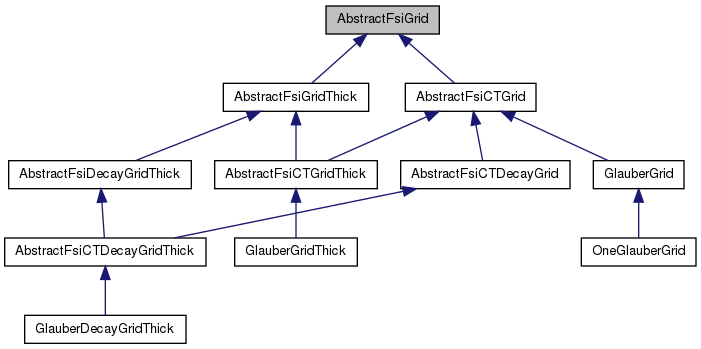
\includegraphics[width=0.9\textwidth]{figs/classAbstractFsiGrid__inherit__graph.png}
\caption{Inheritance diagram of classes in the Glauber library. }
\label{fig:AbstractFsiGrid__inherit__graph}
\end{figure}

An important note is that \texttt{addParticle} and \texttt{addKnockout} are seperate functions that do not call each other. This is done so you can add IFSI particles that are not knock out particles. Or you can exclude particles from contributing to the FSIs. (For example adding a knockout particle that is not actually knocked out in the process will disable the FSIs with this hypothetically knocked out particle).
\subsection{AbstractFsiGridThick}
The \texttt{AbstractFsiGridThick} takes a \texttt{MeanFieldNucleusThick} instead of a \texttt{MeanFieldNucleus} in its constructor. Also makes a \texttt{fsicorrelator} and sets \texttt{number\textunderscore of\textunderscore grids} to 2 and prepends ``Thick.'' to the output grid filenames.
Declares new pure virtual function \texttt{getFsiSrcGridFull\textunderscore interp()} which it uses in the interpolation functions for this grid.

\subsection{AbstractFsiCTGrid}
The \texttt{AbstractFsiCTGrid} sets \texttt{number\textunderscore of\textunderscore grids} to 2. Appends ``.CT.[\textit{hardscale}]'' to the IO filenames.
This one also overloads \texttt{fillGrids()} and \texttt{updateGrids()} to accommodate for the new ``CT'' grid next to the ``regular'' RMSGA grid defined in \texttt{AbstractFsiGrid}. Note that both these still use pure virtual function for actually calculating the grids!

Declares new pure virtual function \texttt{getFsiCtGridFull\textunderscore interp()} which it uses in the interpolation functions for this grid.